\subsection{Linux}
\label{linux}
Als Informatiker befasst man sich oft mit abstrakten und allgemeinen 
Konzepten, die unabhängig von konkreten Betriebssystemen gültig sind. 
Aber sobald man sich an einen Rechner setzt, hat man es dann doch mit 
einem konkreten System zu tun, und innerhalb der Rechnerpools an der Uni
ist dies meist die eine oder andere Linux-Version. Du wirst also im 
Studium nicht drum herum kommen, etwas Erfahrung damit zu sammeln.

Auf deinem eigenen Rechner kannst du natürlich machen,
was immer du möchtest, aber viele von uns bevorzugen auch dort Linux
oder ein anderes Unix-artiges System. Der Umstieg ist gar nicht so
schwer wie man denkt bzw. wie er vor 10 Jahren mal war, und dank Live CDs,
Dual Boot und Virtualisierung kannst du sogar Linux und dein bisheriges 
System parallel laufen lassen und somit ganz unverbindlich reinschnuppern.

\subsubsection{Einstiegshilfen}
Falls du mit Linux bisher keine Erfahrung hast, könnte der Studienbeginn
 der passende Zeitpunkt sein. Die Fachgruppe veranstaltet von Zeit zu Zeit 
Linux-Installationsparties die dir beim Einstieg helfen. Wenn dann im Alltag
irgendein Problem auftritt, ist der nächste Linux-Guru meist nur wenige
Meter entfernt.

Auch wenn du nocht nicht 100\% sicher bist, wohin die Reise geht, solltest 
du also vor dem Kauf eines neuen Rechner sicherheitshalber checken, ob die 
Hardware Linux-Kompatibel ist.

%TODO gibt es eigentlich auch Linux-Kurse, z.B. vom GITZ? Sollte man dann ja hier erwähnen.

\subsubsection{SSH - Zugriff aus der Ferne}
%TODO Hier sollte man auch noch schreiben, wozu das ganze gut ist. Ich kenne SSH und nutze es auch privat, habe mich aber noch nie dazu verannlasst gefühlt, mich mit meinem Uni-Account zu verbinden.
% Auch könnte man einen einleitenden Satz dazu schreiben, was das nun mit Linux zu tun hat.
Um vom heimischen PC aus Zugriff auf deinen Uniaccount zu haben, kannst
du von Linux aus ssh benutzen. F"ur Windowsbenutzer gibt es zwei nette
kleine Tools, Putty und WinSCP. Deinen Uniaccount erreichst du "uber
den Server \nurl{rzstudio.rz.tu-bs.de}.% (xx geht von 01 bis 12).

\begin{description}
\item[Putty] stellt dir eine Shell auf dem UNIX"~Rechner bereit. Damit
kannst du so auf deinem Rechner arbeiten, als w"urdest du direkt auf
dem Server arbeiten (tust du ja auch). Um auch grafische Programme
starten zu k"onnen, musst du noch einen X"~Server f"ur Windows installieren,
z.B. X-Deep32.
\item[WinSCP] ist ein Tool, das einem FTP"~Client "ahnelt. Mit diesem
kannst du Dateien von und zu deinem Uniaccount kopieren. Der Vorteil
ist, dass die "Ubertragung verschl"usselt ist und Passw"orter somit
nicht abgeh"ort werden k"onnen.
\end{description}

Zu allen in diesem Text angesprochenen und noch zu vielen anderen
Computerproblemen mehr gibt es Informationen im Heft "`Don't Panic"',
das kostenlos im Rechenzentrum erh"altlich ist. Nimm es dir gleich mit, wenn
du deine y"~Nummer beantragst.

\subsubsection{Linux-Bezug an der TU-BS}
Fast alle Linux-Distributionen und Softwarepakete für Linux sind freie
Software und somit kostenlos erhältlich.

F"ur Studierende mit Breitband-Internetzugang sind vermutlich die diversen 
Mirror-Server an der Uni interessant. Hier stehen die gr"o"seren 
Distributionen bereit:
	  
\begin{description}
\item[\nurl{ftp://ftp.rz.tu-bs.de/}]~\\Enth"alt Openoffice-, Mozilla-,
Gentoo-, Slackware- und Ubuntumirror, CCC Vortr"age
\item[\nurl{ftp://debian.tu-bs.de/}]~\\Debian-, Kanotix- und Knoppixmirror
\item[\nurl{ftp://ftp.ibr.cs.tu-bs.de/}]~\\Mehr CCC Vortr"age, diverse freie
Software (gr"o"stenteils f"ur Unix/Linux)
\end{description}
%\begin{wrapfigure}{r}{0.5\linewidth}
 %   \begin{center}
  %        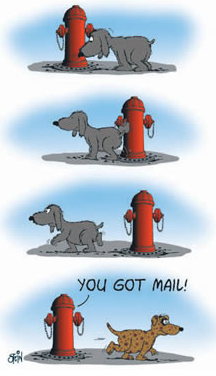
\includegraphics[width=1\linewidth]{bilder/comics/stein2}
%	    \end{center}
%	   %   \caption{A gull}
%	    \end{wrapfigure}
%\begin{wrapfigure}{l}{1.05\linewidth}
 % \vspace{-20pt}
%  \begin{center}
%  \includegraphics%[\linewidth]
%  {bilder/comics/stein2.png}
%\end{center}
%\end{wrapfigure}\ %\newpage
%\vspace{3cm}
F"ur Studierende ohne breitbandigen Netzzugang sind sicherlich die CDs 
n"utzlich, die sich jede/r im
IT Service-Desk\nurlfootnote{http://www.tu-braunschweig.de/it/service-desk}
im Gauß-IT-Zentrum, \nroom{Raum 017}, ausleihen kann. Dort stehen eigentlich
immer die neusten Versionen von SuSE, Mandrake, Fedora, Gentoo, Debian und Knoppix
sowie diverse "altere Distributionen zur Verf"ugung. Dank eines DVD-Brenners
k"onnen inzwischen auch --~soweit vorhanden (SuSE, Knoppix)~-- die
DVD-Versionen verliehen werden. Auf der sicheren Seite ist, wer vorher einen
Abholtermin vereinbart, damit die gew"unschte Distribution garantiert greifbar
ist: 0531/391-5555.
